% ****** Start of file apssamp.tex ******
%
%   This file is part of the APS files in the REVTeX 4.1 distribution.
%   Version 4.1r of REVTeX, August 2010
%
%   Copyright (c) 2009, 2010 The American Physical Society.
%
%   See the REVTeX 4 README file for restrictions and more information.
%
% TeX'ing this file requires that you have AMS-LaTeX 2.0 installed
% as well as the rest of the prerequisites for REVTeX 4.1
%
% See the REVTeX 4 README file
% It also requires running BibTeX. The commands are as follows:
%
%  1)  latex apssamp.tex
%  2)  bibtex apssamp
%  3)  latex apssamp.tex
%  4)  latex apssamp.tex
%
\documentclass[%
reprint,
%superscriptaddress,
%groupedaddress,
%unsortedaddress,
%runinaddress,
%frontmatterverbose,
%preprint,
showpacs,preprintnumbers,
%nofootinbib,
%nobibnotes,
bibnotes,
amsmath,amssymb,
aps,
pra,
%prb,
%rmp,
%prstab,
%prstper,
%floatfix,
]{revtex4-1}

\usepackage{graphicx}% Include figure files
\usepackage{dcolumn}% Align table columns on decimal point
\usepackage{bm}% bold math
\usepackage{booktabs}
%\usepackage{tocloft}
%\usepackage{hyperref}% add hypertext capabilities
%\usepackage[mathlines]{lineno}% Enable numbering of text and display math
%\linenumbers\relax % Commence numbering lines

%\usepackage[showframe,%Uncomment any one of the following lines to test
%%scale=0.7, marginratio={1:1, 2:3}, ignoreall,% default settings
%%text={7in,10in},centering,
%%margin=1.5in,
%%total={6.5in,8.75in}, top=1.2in, left=0.9in, includefoot,
%%height=10in,a5paper,hmargin={3cm,0.8in},
%]{geometry}



\begin{document}

	%\preprint{APS/123-QED}

	\title{Optical Coherence Tomography: \\ Mitigation of Scattering Using DSP Techniques}

	\author{Jared Mann, V00187636}
	\author{Mike Vlanich, V00862757}
	\affiliation{University of Victoria, Faculty of Electrical Engineering}

	\date{\today}% It is always \today, today,


	\begin{abstract}

	\end{abstract}

	%\pacs{Valid PACS appear here}% PACS, the Physics and Astronomy
	% Classification Scheme.
	%\keywords{Suggested keywords}%Use showkeys class option if keyword
	%display desired
	\maketitle
	\tableofcontents

	\makeatletter
	\let\toc@pre\relax
	\let\toc@post\relax
	\makeatother

	\addcontentsline{toc}{chapter}{Contents}
	\listoffigures
	\addcontentsline{toc}{chapter}{List of Figures}
	\listoftables
	\addcontentsline{toc}{chapter}{List of Tables}

	\subsection{\label{sec:level1}		Introduction}
	Optical Coherence Tomography (OCT) is a non-invasive method of producing 2-Dimensional images of internal tissues in a method comparable to that of ultrasound imaging.\cite{Huang91}\cite{sander_optical_2011} The practice came into prominence following the developments of Huang et al. at the Massachusetts Institute of Technology in 1991. \cite{Huang91}




	\section{\label{sec:level1}OCT Identified Problem and Suggested Solution}
	\subsection{\label{sec:level2} The Problem of Speckle Noise}
	\begin{figure}
		\centering
		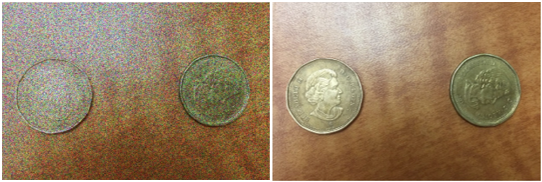
\includegraphics[width=0.7\linewidth]{Figures/specklefilter2}
		\caption{On the left is an image put through a speckle filter in Matlab. On the right is the original image.}
		\label{fig:specklefilter2}
	\end{figure}
	A problem with using an OCT interferometer is that ‘speckle’ noise exists, which ultimately reduces the quality of the image. Speckle is a phenomenon that is caused by interference of the reflected wave at the photo-detector. Speckle noise is evident when trying to image non-fluid structures (such as hard tissue). As the wave propagates it becomes distorted due to “low-angle multiple forward scattering and diffuse multiple backscattering of coherent photons”. \cite{Popescu2007}

	In OCT interferometry imaging, photons are detected after one backscattering event for most relevant information, but when a wave is propagated through a dense biological sample it experiences numerous scattering events (in OCT interferometry). These scattering events increase the likelihood for photons to change their travel distance comparative to their airborne path which results in speckle noise reducing the image quality. \cite{Popescu2007}



	\subsection{\label{sec:level2} Possible Solutions for Speckle Noise}
	As technology progress in imaging processing, techniques are being developed to help reduces the effects of speckle noise when using OCT. Some of these methods include decreasing spatial and temporal coherence of the laser used. While more trivial techniques such as phase-domain processing and zero-adjustments are used to improve image quality due to speckle noise. \cite{Popescu2007}
	\section{\label{sec:level1} Conclusion}
	The progression of OCT in the field of ophthalmology has been instrumental in diagnosing patients with retinal diseases for many years. The ability to clearly image the eye 2-dimensionally while being non-invasive has provided great insight in monitoring and identifying certain patterns of diseases for early preventative and diagnostic actions. Although using OCT is promising in fluid filled samples, imaging of denser biological samples induces noise due to numerous backscattering events. As digital signal processing advances the speckle noise could be reduced and OCT interferometry could be implemented to a deeper degree of imaging biological tissues. Techniques such as compounding spatially displaced OCT images, understanding the characteristics of the tissue, and using algorithms such as wavelet filtering, phase domain processing and median filtering are possible solutions to the problems introduced by scattering.\cite{Popescu2007}. As scientists continue to develop theoretical knowledge and analysis, while technology improves, optimism is increased in the development of OCT imaging. AND HOW.




	\bibliographystyle{apa}
	\bibliography{apssamp}% Produces the bibliography via BibTeX.

\end{document}
%
% ****** End of file apssamp.tex ******
